\section{Présentation du projet}
 
\paragraph{}
Nous avons proposé notre propre projet dans l’optique de créer un jeu pour téléphone mobile, de sa conception jusqu’à sa mise en ligne. Le concept de base est de créer un “jeu de rythme”, à l'aide du moteur de jeu Unity. Nous nommerons notre jeu \textbf{Heliko} (Escargot en Espéranto).
 
\paragraph{}
La difficulté relève dans un grand travail de recherche : le jeu doit être intéressant et réalisable afin de pouvoir le mettre en ligne dans le temps donné. La méthode de gestion de projet avait une grande importance.
 
\begin{figure}[H]\centering
  
\includegraphics[scale=1]{./img/game.png}
  \caption{Extrait du jeu final}
  \label{game}
\end{figure}
 
\section{Analyse de départ}
 
\paragraph{}
Nous avons dès le départ conçu les parties du jeu pour qu’il soit jouable et en ligne au bout de 4 mois de travail. Étant donné notre légère expérience dans la gestion du temps, nous avons conçu des “couches” à développer pour former le jeu de façon incrémentale et ainsi être certain d’aboutir à un résultat (à condition de prendre en compte les tests, les finitions et la mise en ligne).
 
\paragraph{Couches incrémentales}
\begin{enumerate}
\item Créer un moteur de jeu de rythme Unity générique et créer un mini jeu jouable sur Android ;
\item Rendre l’application jouable sur tous les mobiles et supports ;
\item Créer d’autres mini jeux ;
\item Créer un moteur de tutoriel et les tutoriels associés ;
\item Concevoir et ajouter une monétisation (gain de pièces dans les niveaux, et personnalisation du jeu) ;
\item Concevoir et ajouter un esprit communautaire (partage de l’avancement) ;
\item Créer un éditeur public de niveaux contributif.
\end{enumerate}
 
\paragraph{}
Le projet est sous-divisé en trois grandes étapes :
\begin{itemize}
\item Conception et prototypes ;
\item Développement du jeu ;
\item Tests, finitions et mise en ligne (Play Store et Apple Store).
\end{itemize}
 
\paragraph{}
Ces 3 étapes demandant une gestion de projet différente, la méthode de travail a été modifiée au fil du développement.
 
\paragraph{}
Le \textbf{diagramme de Gantt} initial a été conçu dans l’optique de faire la totalité des couches énoncées plus haut.
 
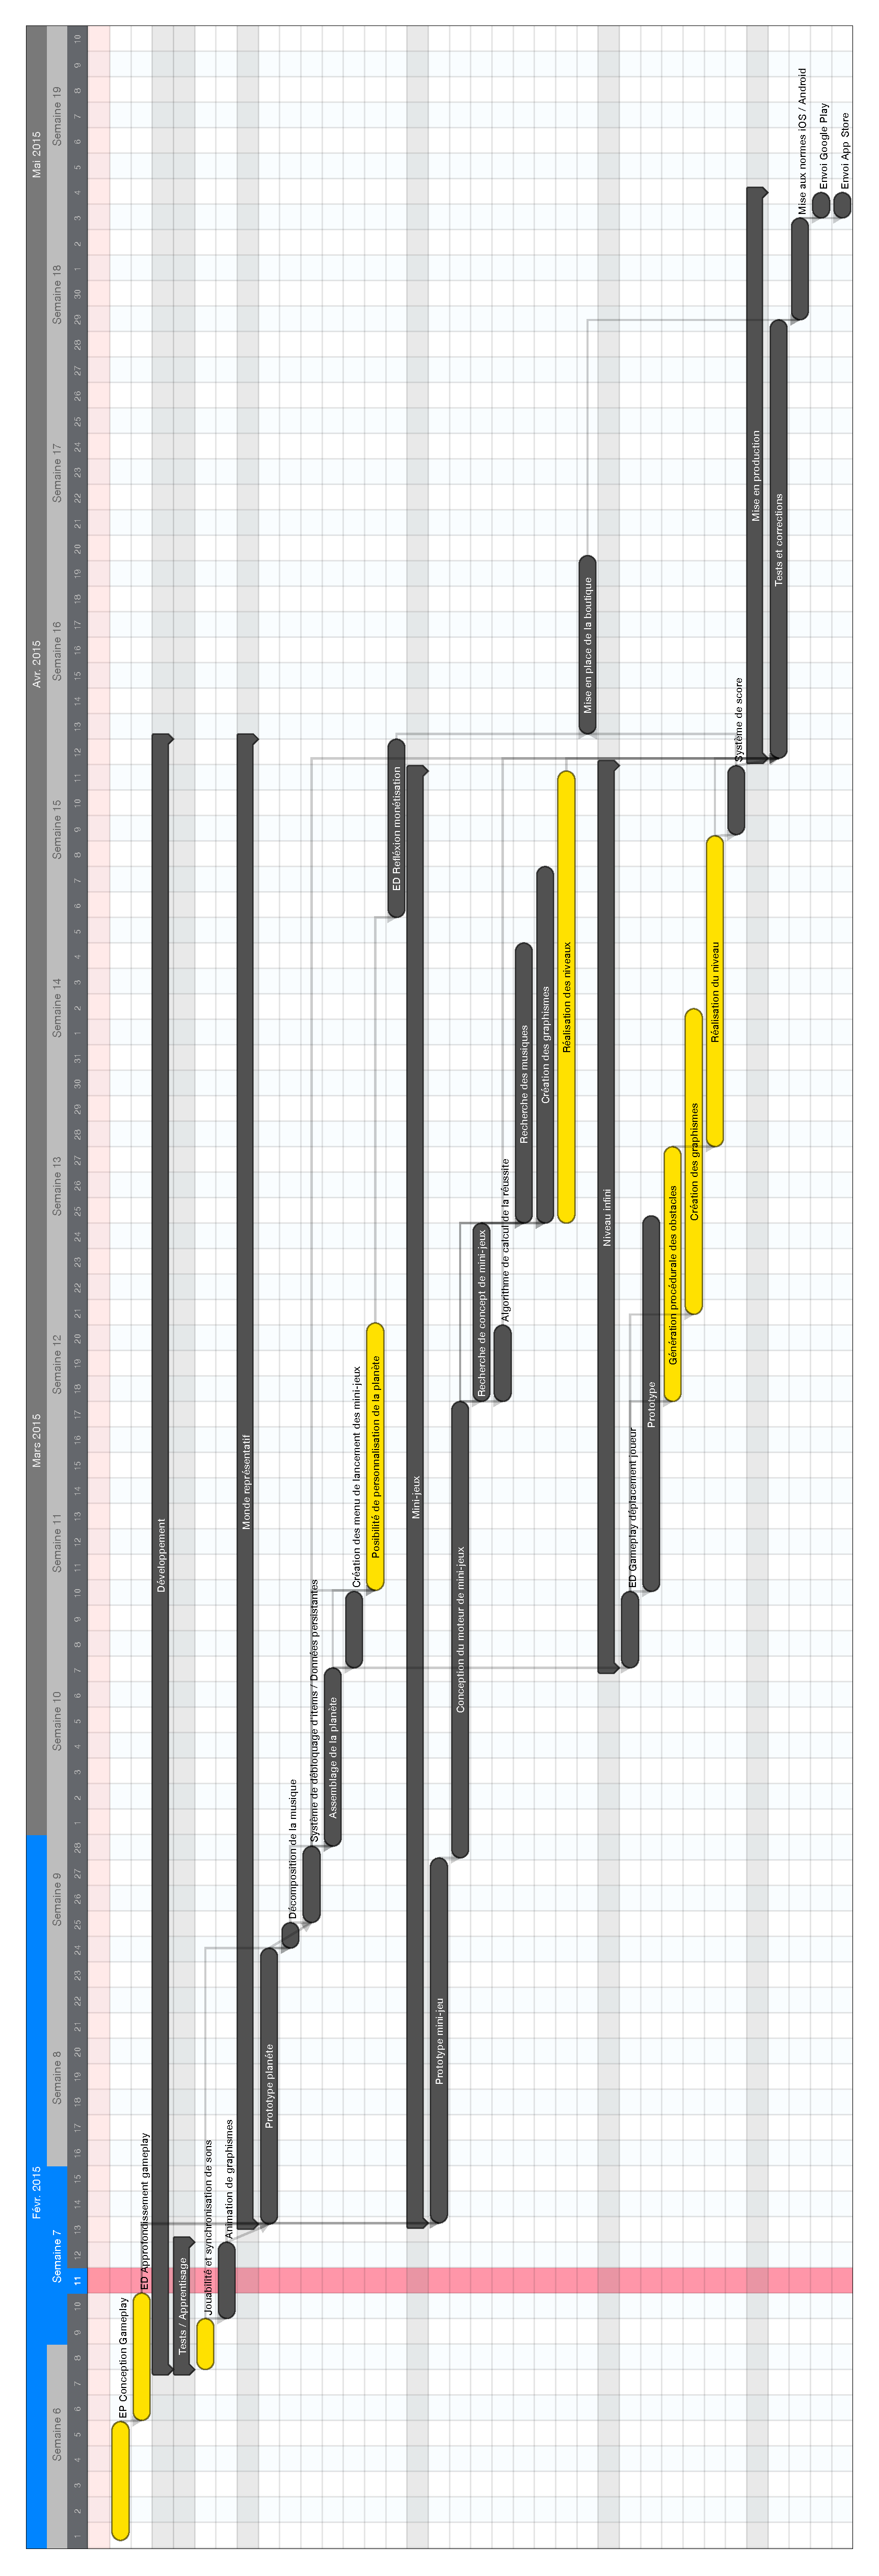
\includepdf{oufGantt3.pdf}
 
\paragraph{Rôles dans l’équipe}
Vu la charge importante de travail et la diversité des tâches, nous avons préféré nous attribuer des responsabilités fixes :
 
\begin{itemize}
\item \textbf{Stéphane Wouters}, chef de projet ;
\item \textbf{Noé Le Philippe}, responsable développement technique ;
\item \textbf{Thibaut Castanié}, responsable son et graphismes ;
\item \textbf{Jolan Konig}, responsable intégration et publication.
\end{itemize}
 
\paragraph{}
Nous avons fait le choix de travailler ensemble sur toutes les parties, et nous nous sommes affectés, au fil du projet, des micro tâches.
 
\section{Outils et méthode de travail}
 
\subsection{Gestionnaire de tâches}
 
\paragraph{}
Pour faire avancer le projet, nous avons utilisé toutes les capacités d’un gestionnaire de tâches en ligne, \textbf{Trello}, qui est un outil inspiré par la \textit{méthode Kanban}. Nous nous sommes imposé de visiter ce tableau tous les jours et ses outils de notifications nous ont permis d’être continuellement connectés.
 
\paragraph{}
Trello permet une gestion des tâches dans le Cloud avec de nombreuses fonctionnalités :
\begin{itemize}
\item Création de tâches, avec titre et description ;
\item Choix d’une date de fin sur une tâche ;
\item Affectation de membres à une tâche ;
\item Labels (tags) personnalisés ;
\item Commentaires sur chaque tâche pour discussion asynchrone entre les membres du groupe sur une tâche ;
\item Application Android et iOS avec notifications par \textit{push}.
\end{itemize}
 
\paragraph{}
Un système de rangement vertical a été adopté pour les types de tâches, et des labels de couleurs en fonction de l’avancement des tâches :
 
\begin{itemize}
\item \textbf{Bloquante} (tâche à réaliser rapidement, bloquant l’avancement du projet) ;
\item \textbf{À discuter / en recherche} (tâche en cours de discussion, pour prise de décision) ;
\item \textbf{À attribuer} (Tâche correctement spécifiée, en attente d’affectation à un membre de l’équipe ;
\item \textbf{En réalisation} (tâche en cours de réalisation par un ou plusieurs membres de l’équipe) ;
\item \textbf{À tester / à contrôler} (tâche réalisée, à tester pour confirmation) ;
\item \textbf{Fait} (tâche réalisée et fonctionnelle, prête à être archivée).
\end{itemize}
 
\paragraph{}
Les tâches sont classées dans des colonnes “TODO” triées par thèmes (développement, graphismes…), ou par cycle itératif (d’un jour à une semaine).
 
\begin{figure}[H]\centering
  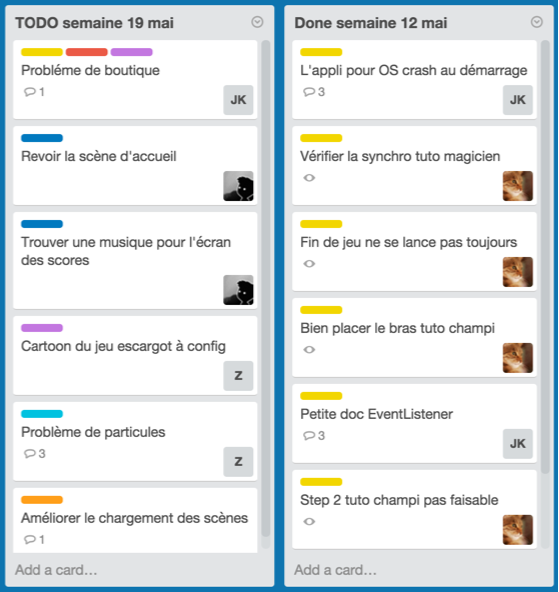
\includegraphics[scale=1]{./img/trello.png}
  \caption{Exemple de colonnes en fin de projet}
  \label{trelloc}
\end{figure}
 
\paragraph{}
Trello a aussi été utilisé comme mémo et pour archiver les ressources graphiques et sonores (figure \ref{trellomemo}).
 
\begin{figure}[H]\centering
  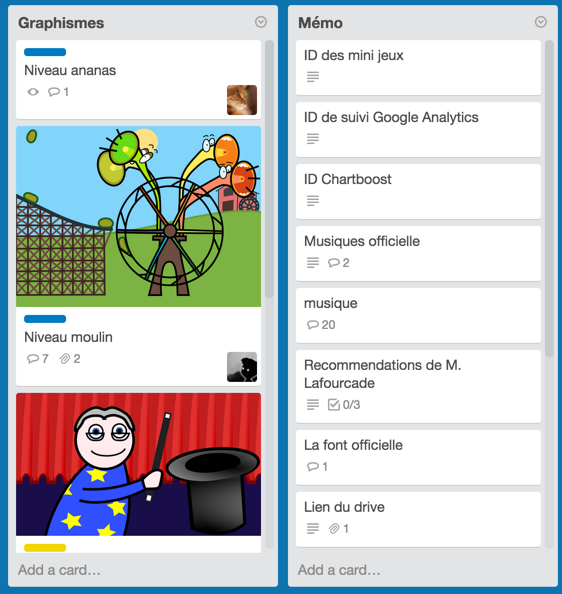
\includegraphics[scale=1]{./img/trello_autres.png}
  \caption{Utilisation de Trello comme mémo et archives}
  \label{trellomemo}
\end{figure}
 
\paragraph{}
Cette méthode de travail avec Trello nous a permis d’être efficace 100\% du temps au travers d'Internet. Il n’y avait jamais de temps mort et nous étions toujours clairs dans notre direction tant que quelqu’un (chef de projet) s’occupait de créer des tâches et de les organiser.
 
\subsection{Réunions}
 
\paragraph{}
Même si \textit{Trello} nous permet de travailler de façon indépendante, nous nous sommes réunis très régulièrement pour travailler ensemble et fixer les nouveaux objectifs, une à quatre fois par semaine.
 
\paragraph{}
Pendant les longues séances de travail en collaboration (de 9h à 18h par exemple), nous avons utilisé un véritable tableau blanc pour noter les tâches en cours et les affectations. Exemples de tâches :
 
\begin{itemize}
\item Réadapter la taille du logo \textit{pause} sur Android v4.1 en écran 16:10 ;
\item Couper les 150ms du début du son \texttt{tic.wav} ;
\item Revoir l’animation du bras gauche du champignon.
\end{itemize}
 
\paragraph{}
Les tâches étant à 80\% de ce type (courtes et rapides), l’organisation est très importante pour être efficace.
 
\paragraph{}
De nombreuses heures de réunion étaient dédiées à la recherche de concept ou de remise en question des objectifs. Par exemple abandonner le développement d’un mini jeu trop complexe, ou en inventer de plus simples.
 
\subsection{Cycles itératifs}
 
\paragraph{}
Dès le départ, un développement par cycles itératifs a été choisi. Bien adapté pour le développement d’un jeu vidéo et surtout à cause de notre contrainte principale : notre liberté sur les choix.
 
\paragraph{}
Les premières semaines ont été dédiées à la réalisation de prototypes et de tests en augmentant toujours la difficulté, dans l’objectif de produire un moteur de jeu de rythme fonctionnel qui correspond aux besoins définis dans le cahier des charges.
 
\begin{itemize}
\item \textbf{Prototype 1} - Réalisation d’un cube qui bat à un rythme constant (3 jours)
\item \textbf{Prototype 2} - Réalisation d’un prototype de test de réussite (2 jours)
\item \textbf{Prototype 3} - Création de la première version du moteur de rythme (6 jours)
\item \textbf{Prototype 4} - Réalisation d’un prototype d’animations, connectés au moteur de rythme (4 jours) \emph{-> Le moteur n’est pas assez précis et doit être revu}
\item \textbf{Prototype 5} - Deuxième version du moteur de rythme (3 jours)
\item \textbf{Prototype 6} - Nouvelle tentative de connexion à des animations (1 jour) \emph{-> Test OK. On s’aperçoit que nous avons besoin de quart de temps dans le modèle et qu’il faut recommencer une nouvelle fois sa conception}
\item \textbf{Prototype 7} - Troisième version du moteur de rythme (4 jours)
\item Etc.
\end{itemize}
 
\begin{figure}[H]\centering
  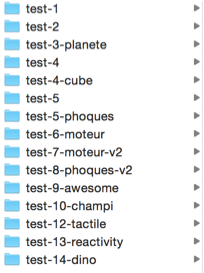
\includegraphics[scale=1]{./img/list-tests.png}
  \caption{Les différents projets Unity de tests}
  \label{listte}
\end{figure}
 
\paragraph{}
On voit sur la figure \ref{listte} l'ensemble de nos tests. A chaque nouveau test, un nouveau projet Unity. Au \textbf{test 14}, nous avons jugé que le moteur correspondait à nos attentes et nous avons ensuite itéré directement sur ce projet. C’est à ce moment (environ 1 mois après le début du projet) que le système de fonctionnement à changé et que nous avons fonctionné en micro tâches.
 
\paragraph{}
Les dernières semaines ont été dédiées aux finitions sur le projet afin de rendre le jeu agréable avec un aspect “fini”.
 
\subsection{Github}
 
\paragraph{}
Un gestionnaire de version pour notre projet a bien sûr été utilisé et nous avons choisi le gestionnaire \emph{Github} qui offre de nombreux outils de statistiques très intéressants.
 
\paragraph{}
Déjà habitués à Git, nous l'avons utilisé pleinement et nous avons envoyé des \emph{commits} pour chaque modification fonctionnelle. Nous sommes ainsi arrivés en fin de projet avec un cumul de plus de \textbf{980 commits}, globalement bien répartis entre nous quatre. (Avec plus de 2 millions de modifications dans les fichiers...).
 
\begin{figure}[H]\centering
  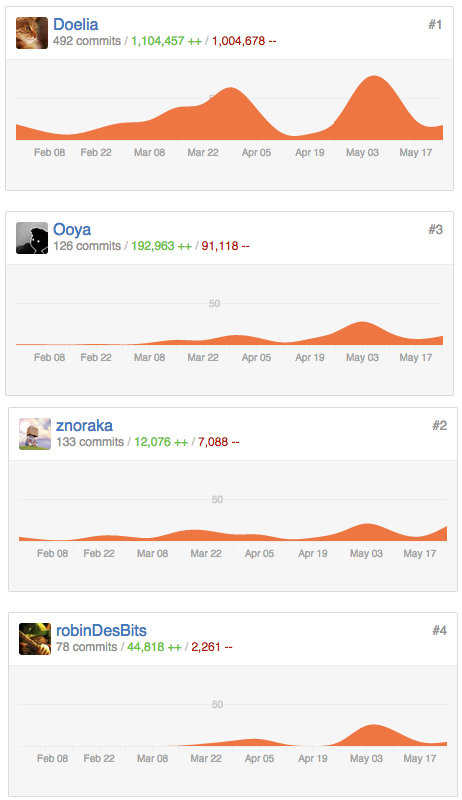
\includegraphics[scale=.5]{./img/github_commits.png}
  \caption{Répartition des commits dans le temps}
  \label{github_commits}
\end{figure}
 
\paragraph{}
On remarque d'après la figure \ref{github_commits} de nombreuses suppressions (presque autant que d’additions), prouvant l’évolution du projet et l’application des cycles itératifs. Le développement s’est fait continuellement dans le temps.
 
\subsubsection{Ponctualité hebdomadaire}
 
\begin{figure}[H]\centering
  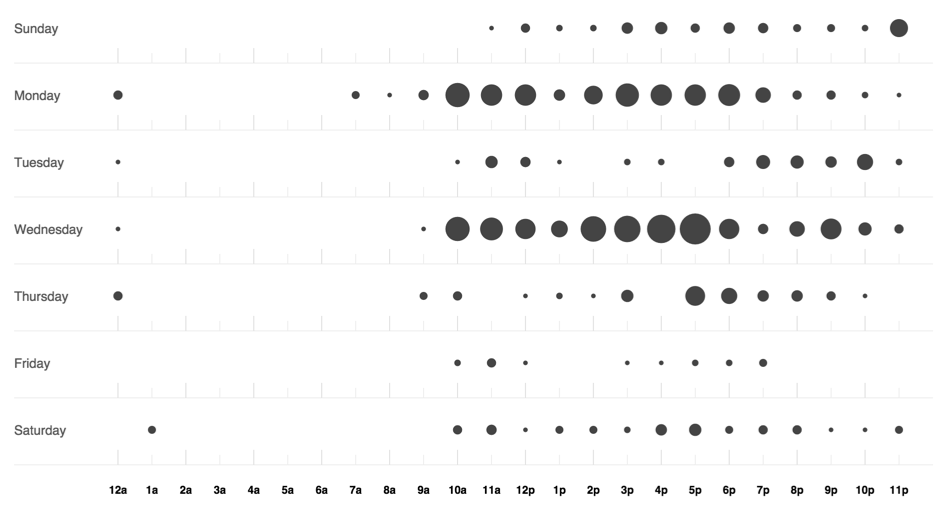
\includegraphics[scale=.8]{./img/punchcard.png}
  \caption{Punch card de Github}
  \label{punchcard}
\end{figure}
 
D’après les statistiques \emph{Github} (figure \ref{punchcard}), nous avons travaillé tous les jours de la semaine, avec une préférence pour le lundi et le mercredi en après-midi et jusqu’en fin de soirée.
 
 
\subsubsection{Modélisation Gource}
 
Gource est une application qui permet de tracer en vidéo l’historique des commits qui construit l’architecture des fichiers d’un projet GIT.
 
\paragraph{}
Cette capture (figure \ref{gource_over}) représente l’état final de l’architecture des fichiers du projet. La taille de la branche des tests démontre qu'ils ont effectivement constitué une grande partie du projet (Environs 30\%).
 
\begin{figure}[H]\centering
  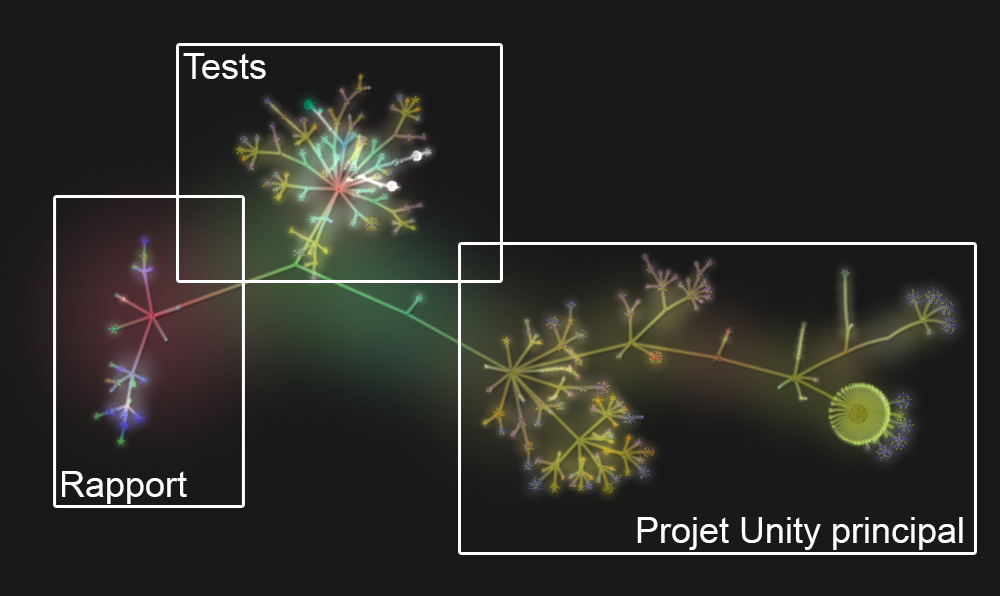
\includegraphics[scale=.3]{./img/gource_over.png}
  \caption{Modélisation Gource en fin de projet}
  \label{gource_over}
\end{figure}
 
\section{Estimation du temps passé}
 
\paragraph{Estimation globale}
Nous nous sommes réunis au moins une fois par semaine pour travailler, sur des séances d'environ 8h sur une journée. Sur 4 mois, cela représente un total de 128 heures par personnes, et 512 heures au total. A cela nous pouvons y ajouter toutes les heures de travail individuels, que nous chiffrons facilement à 30\% du projet. Soit \textbf{665 heures} au total.
 
\paragraph{Estimation assistée}
Étant donné que nous envoyons très régulièrement des commits, nous avons essayé d'utiliser un outil de calcul :  \textbf{git-hours}. Il calcule les heures de travail en fonction des écarts entre les commits. (Mais ne compte évidemment que le temps de développement pure, les moments passés à discuter et débattre autour du projet en équipe ne sont donc pas comptabilisés. L'application retourne un total de \textbf{29822} minutes, soit \textbf{497 heures}. Ce qui semble totalement cohérent avec notre première estimation, en ajoutant les heures de débats en réunion.
 
\paragraph{Conversion en jours/hommes}
En prenant une base de 35h par semaines, cela représente un travail de \textbf{133 jours/homme} \textit{(665/35 * 7 jours)}.
 
 
\section{Résultat et comparaison avec le prévisionnel}
 
\paragraph{}
Globalement à 2 semaines avant la date finale, on peut admettre que l'objectif a été atteint.
Le jeu est jouable et tout est prêt pour qu'il soit mis en ligne sur l'Apple Store et le Play Store. Les tests auprès des utilisateurs ont été concluants.
 
\paragraph{}
La liste des \textit{couches} (prévues dans l'analyse) qui ont été développées est la suivante :
\begin{itemize}
\item 3 mini jeux pleinement fonctionnels ;
\item Des tutoriels pour chacun des mini jeux ;
\item Jeu jouable sur tous les téléphones sous Android et iOS ;
\item Système de déblocage des mini jeux et enregistrement du taux réussite ;
\item Monétisation avec de la publicité.
\end{itemize}
 
\paragraph{}
Les éléments suivants n'ont pas été développés, par choix :
\begin{itemize}
\item Système de personnalisation ;
\item Mode de jeu infini répétitif ;
\item Éditeur de niveau collaboratif.
\end{itemize}
 
\paragraph{}
Ces choix de retrait se sont faits suffisamment tôt dans le projet (à mi-parcours pour être certain d'aboutir à un jeu fonctionnel). Nous avons préféré nous concentrer sur les tâches listées ci-dessus. Ce fut tout de même un travail important.
 
\paragraph{}
Nous sommes globalement satisfaits de notre gestion du temps, et nous pensons que notre organisation y a beaucoup contribué.
L'expérience de créer un jeu de A à Z nous a beaucoup appris et nous a permis de mettre en oeuvre beaucoup de concepts sur la gestion de projets.